
This chapter



%======================================================
\section{Characterizing \aclp{DTE}}
\label{sec:ecosystems}
%======================================================

As discussed in \Cref{sec:background}, the \ac{DT} concept is shifting from ultra-detailed replicas of individual \acp{PA} to contextualized models tailored to specific applications~\cite{minerva2020dtiot}.
%
However, many solutions either mirror isolated assets -- overlooking their interrelations -- or adopt monolithic models for complex systems (e.g., entire cities~\cite{Deren2021}).
%
In this paper, we focus instead on the idea of modeling such large-scale scenarios using what we informally define as a:

% \newtheorem*{dte}{Digital Twin Ecosystem}
% \begin{dte}
%     A dynamic set of \aclp{DT}, each representing a \ac{PA}, whose meaningful relationships within a target context make it valuable to consider their collective evolution to accurately reflect the mirrored portion of the physical world.
% \end{dte}

In order to characterize \acp{DTE}, in this section,
we analyze the challenges surfacing from the heterogeneity of complex domains (\ref{rq:dimensions})
and provide an operational definition of \acp{DTE} in terms of functionalities and services that consumers may expect to use (\ref{rq:functionalities}).
Finally, we compare architectural approaches for \acp{DTE} by investigating the state of the practice (\ref{rq:implementations}).


%=======================================================
\section{Operational Characterization}
\label{sec:operational-characterization}
%=======================================================

To better characterize the concept of \ac{DTE}, we analyze the fundamental functionalities to ease the fruition of services that span across several \acp{DT}.
%
We intend this operational definition to be general, regardless of the architectural design adopted to develop the ecosystem.

We consider the perspective of both \emph{managers} of the \ac{DTE} who need to oversee the creation and evolution of the ecosystem, and \emph{consumers} who instead are interested in exploiting the \ac{DTE} abstraction for their application goals.
%
We will then let these functionalities guide our implementation proposal that we describe in \Cref{sec:hwodt-idea}.

\subsubsection{Managing the \ac{DTE}}\label{sssec:operational-managing}

We define \ac{DTE} as a \emph{dynamic} set of \acp{DT} as members could join or leave the ecosystem at any time due for different reasons.
These include the \acp{PA} lifecycle (e.g., decommissioning) or application-specific inclusion criteria adopted when modeling the ecosystem (e.g., entering or exiting a geographical area).
%
To support this dynamism, \acp{DTE} should provide operations to \emph{add} and \emph{remove} \acp{DT}.
These can be public or restricted to administrators, and invocations can be either manual or automatically triggered by monitoring processes (or the \acp{DT} themselves) when detecting relevant changes in the physical environment.

A consequence of this dynamic management is the need to easily \emph{discover} which \acp{DT} are part of the ecosystem.
\acp{DTE} may hold an index of all (currently) registered \acp{DT}, each \emph{uniquely identified} and described with metadata to support fine-grained discovery.
%
A key piece of information to store is the mirrored \ac{PA} identifier, allowing tracking of both the digital and physical components of the ecosystem.
As noted in \Cref{ssec:dimensions}, since multiple \acp{DT} may represent the same \ac{PA} for different purposes, this information becomes especially valuable.
Moreover, to keep track of a \ac{DT} evolution, it should be possible to \emph{update} metadata over time.

\subsubsection{Exploiting the \ac{DTE}}\label{sssec:operational-exploiting}

\emph{Consumers} of a \acp{DTE} represent either human users, applications, or intelligent agents~\cite{burattini2025iot} which may be interested in observing the state of the registered \acp{DT} and exploiting their services.
%
An ecosystem should then offer functionalities to access individual \acp{DT} and ecosystem-wide services. 

This includes the ability to retrieve the current \emph{representation} of the state of all \acp{DT} and their relationship at a given time.
%
As the representation could grow very large, it can be more effectively managed by enabling consumers to \emph{query} the ecosystem, enabling them to select and aggregate relevant data across multiple \acp{DT}.
%
This supports the derivation of insights that would not be easily discovered by accessing each \ac{DT} individually.

Finally, given the dynamic nature of \acp{DT} continuously updating their representation of the corresponding \acp{PA}, \acp{DTE} should support \emph{observation} patterns -- even selectively through continuous queries~\cite{babu2001sigmod} -- to track changes of \acp{DT} and of the whole ecosystem over time.

Although not an operation provided by the ecosystem itself, we include \emph{navigation} by following \ac{DT} relationships as a fundamental feature of \acp{DTE} complementing the other interaction patterns.
%
This allows users to explore and discover information progressively.
Moreover, relationships may cross ecosystem boundaries, offering paths to discover related \acp{DTE}.

%=======================================================
\section{Architecting \aclp{DTE}}
\label{sec:architecting-dte}
%=======================================================

\begin{figure}[t]
    \centering
    \begin{subfigure}[b]{0.3\linewidth}
        \centering
        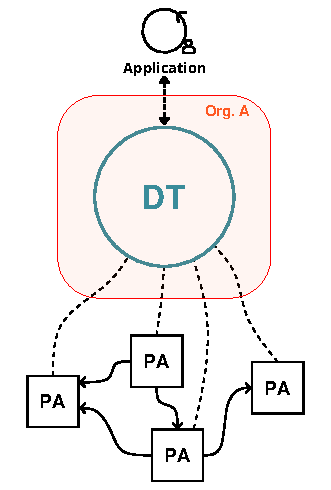
\includegraphics[width=\linewidth]{figures/hwodt/ecosystems_types-monolithic.pdf}
        \caption{\textbf{Monolithic} \ac{DTE}}
        \label{fig:ecosystem-monolithic}
    \end{subfigure}
    \hfill
    \begin{subfigure}[b]{0.3\linewidth}
        \centering
        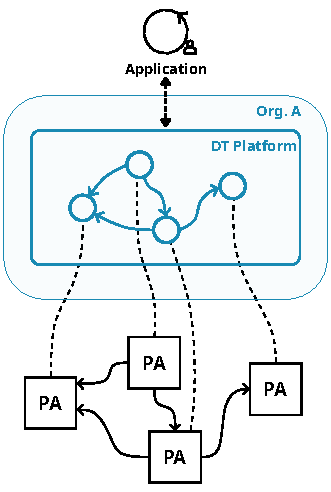
\includegraphics[width=\linewidth]{figures/hwodt/ecosystems_types-homogeneous.pdf}
        \caption{\textbf{Homogeneous} \ac{DTE}}
        \label{fig:ecosystem-homogeneous}
    \end{subfigure}
    \hfill
    \begin{subfigure}[b]{0.3\linewidth}
        \centering
        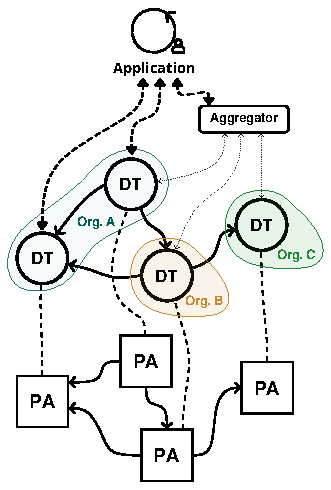
\includegraphics[width=\linewidth]{figures/hwodt/ecosystems_types-heterogeneous.pdf}
        \caption{\textbf{Heterogeneous} \ac{DTE}}
        \label{fig:ecosystem-heterogeneous}
    \end{subfigure}
    \caption{Three architectural approaches for \acp{DTE}: in \ref{fig:ecosystem-monolithic} a single \ac{DT} models the whole scenario; in \ref{fig:ecosystem-homogeneous} a single platform is used to build and deploy all the \acp{DT} in the ecosystem; in \ref{fig:ecosystem-heterogeneous} maximum flexibility is allowed, possibly reusing existing \acp{DT} under a common interface.}
    \label{fig:ecosystem-types}
\end{figure}

This section analyzes and compares approaches from current practice in applying \acp{DT} to complex scenarios involving multiple \acp{PA}.
We focus on four aspects derived from our \ac{DTE} characterization in terms of heterogeneity and operational behvior:
\begin{inlinelist}
\item the degree to which the ecosystem can evolve to reflect physical-world changes (\emph{evolvability}),
\item whether they support heterogeneous \acp{DT} within the same ecosystem (\emph{heterogeneity}),
and 
\item whether ecosystem-level functionalities are offered to users (\emph{services}).
\end{inlinelist}

We reviewed relevant works from the state of the art, survey papers, and technical documentation of \ac{DT} frameworks and platforms.
Although not a systematic review, our analysis shows three main emerging architectural approaches to implement \acp{DTE}.
%
We name these patterns \emph{monolithic}, \emph{homogeneous}, and \emph{heterogeneous} \acp{DTE}, and we schematically show their different architectures in \Cref{fig:ecosystem-types}.
We summarize our feature comparison in \Cref{tab:comparison-summary} and discuss the main peculiarities of each approach below.


\note{table}
% \noindent
% \begin{table}[t]
%     \centering
%     \begin{tabular}{l|c|c|c}
%     \toprule
%     \midrule
%     \textbf{} & \textbf{Mon.} & \textbf{Hom.} & \textbf{Het.} \\
%     \hline
%     \hline
%     \textit{Evolvability} & $\times$ & \checkmark & \checkmark
%     \\
%     \hline
%     \textit{Heterogeneity} & $\times$ & $\times$ & \checkmark
%     \\
%     \hline
%     \textit{Services} & \checkmark & \checkmark & \checkmark
%     \\
%     \hline
%     \bottomrule
%     \end{tabular}
%     \caption{Comparison summary of Monolithic (Mon.), Homogeneous (Hom.), and Heterogeneous (Het.) \acp{DTE} that shows supported (\checkmark)
%     %partially supported ($\sim$),
%     and not supported ($\times$) features.}
%     \label{tab:comparison-summary}
% \end{table}

\subsubsection{Monolithic \acl{DTE}}
\label{sssec:monolithic}

The most straightforward approach is to model the entire targeted context as a single, monolithic \ac{DT}.
Due to the fuzzy definition of a \ac{PA}, even complex entities (e.g., an entire city) can serve as valid physical counterparts of a single \ac{DT}, with some models explicitly capturing multiple internal components of such entities.

The main benefit of this approach is its simplicity in deriving the overall system architecture:
all physical-world data can flow into a single system built with a consistent technological stack (\Cref{fig:ecosystem-monolithic}).
%
A monolithic \ac{DT} also offers strong modeling capabilities and facilitates services such as running simulations on a single model of the entire ecosystem.

The drawbacks of the approach are on the management side. Representing with high fidelity dynamic scenarios involving multiple heterogeneous assets can be challenging, and even minor updates -- such as adding new entities or modifying the behavior of existing ones -- may require modifying the entire \ac{DT}.
%
This approach is not suited for rapidly evolving ecosystems or contexts involving multiple stakeholders.
%
Relying on a single \ac{DT} limits technological diversity and prevents the reuse of existing \acp{DT}, forcing the creation of a new, unified model.

Examples of monolithic \acp{DT} include modeling a single \ac{DT} for entire roads~\cite{KUSIC2023101858}, hospital buildings~\cite{dt_hospital}, or smart grids~\cite{9449682}. 

\subsubsection{Homogeneous \acl{DTE}}
\label{sssec:homogeneous}

We refer to \emph{homogeneous} \acp{DTE} when the approach relies on a general-purpose platform that natively supports the definition of multiple \acp{DT} (\Cref{fig:ecosystem-homogeneous}).
%
The \ac{DT} are hence homogeneous in their modeling and implementing technology as they are created within the same platform.
%
The native support for \acp{DTE} enhances adaptability to the evolving physical world as it is simple to add and remove \acp{DT} or update models.
%
Furthermore, the modeling and technological homogeneity make implementing ecosystem services relatively easy, as in the \emph{monolithic} approach.
%
Differently, though, it is possible to highlight the individuality of the involved \acp{DT}, which may independently process the relative data flows, offering better decomposition and separation of concerns.

However, the dependency on a single model and platform may introduce vendor lock-in, modeling and organizational constraints, limiting support for heterogeneous \acp{PA}.

An example of this approach is the Azure Digital Twins platform, which introduced the concept of a \emph{Twin Graph}\footnote{\url{https://learn.microsoft.com/en-us/azure/digital-twins/concepts-twins-graph}} to explicitly represent relationships among \acp{DT} modeled using a uniform \ac{DTDL}.


\subsubsection{Heterogeneous \acl{DTE}}
\label{sssec:heterogeneous}

The third approach is based on introducing a common interoperability layer on top of heterogeneous \acp{DT}.
%
By embracing the inherent heterogeneity of \acp{DTE}, it enables the reuse of existing \acp{DT} while ensuring uniform access and navigation for consumers (\Cref{fig:ecosystem-heterogeneous}).
%
\acp{DT} are implemented as standalone software components, each with specific models and technologies, and each exposing interfaces that can be used by applications directly or through intermediary aggregators.

This approach is well-suited for dynamic, open \acp{DTE} where \acp{DT} are developed by various stakeholders since the individual components are loosely coupled.
%
Furthermore, \acp{DT} are not limited to being part of only one ecosystem, granting an additional degree of flexibility.

To maintain interoperability, though, each \ac{DT} must be mapped to a shared metamodel to represent it within the ecosystem and expose a shared interface to enable seamless interaction.
This can lead to a potential loss of information and expressivity, as with any model conversion.
However, direct access to the original \ac{DT} remains possible when needing to use specialized services not easily mapped in the shared model.

Compared to previous approaches, where services are typically provided by the implementing technology/platform and benefit from modeling uniformity, implementing ecosystem-wide services in heterogeneous \acp{DTE} is inherently more complex.
%
This can be achieved through either fully distributed techniques
-- such as polystores~\cite{dggan2015polystore} or federated and link-traversal queries~\cite{schwarte2011semweb,quilitz2008querydistributed,bogaerts2021linktraversalquery} --
or by introducing a middleware (as shown in \Cref{fig:ecosystem-heterogeneous}) aggregating \acp{DT} and implementing the required functionalities.
%
This doubles as a way to set a clear boundary for operations, allowing a clear definition of which \acp{DT} belong to an ecosystem.

In this paper, we demonstrate how such an interoperability layer and ecosystem services can be implemented using Web technologies and standards, paving the way for the realization of open heterogeneous \acp{DTE}.

To make a parallel with open Web-based ecosystems, this would be similar to a web service exposing a well-documented public HTTP API, which does not prevent specialized consumers from using remote method invocation if they have specialized knowledge on how to interact with the server.

For the approach to be successful and encourage \ac{DT} developers to join heterogeneous ecosystems, the entry barrier needs to be set at a relatively low level to ensure take-up, while still maintaining a sufficient level of complexity to meet the overall objectives~\cite{kendall2021ndt}.

